
%!TEX encoding = UTF-8 Unicode
% !TeX spellcheck = en_GB


%%%%%%%%%%%%%%%%%%
%\appendix
%%%%%%%%%%%%%%%%%%%

%%%%%%%%%%%%%%%%%%
\section{Discussions on EW fits}
\label{app:EW}
%%%%%%%%%%%%%%%%%%

\begin{figure}[t]
	\centering
	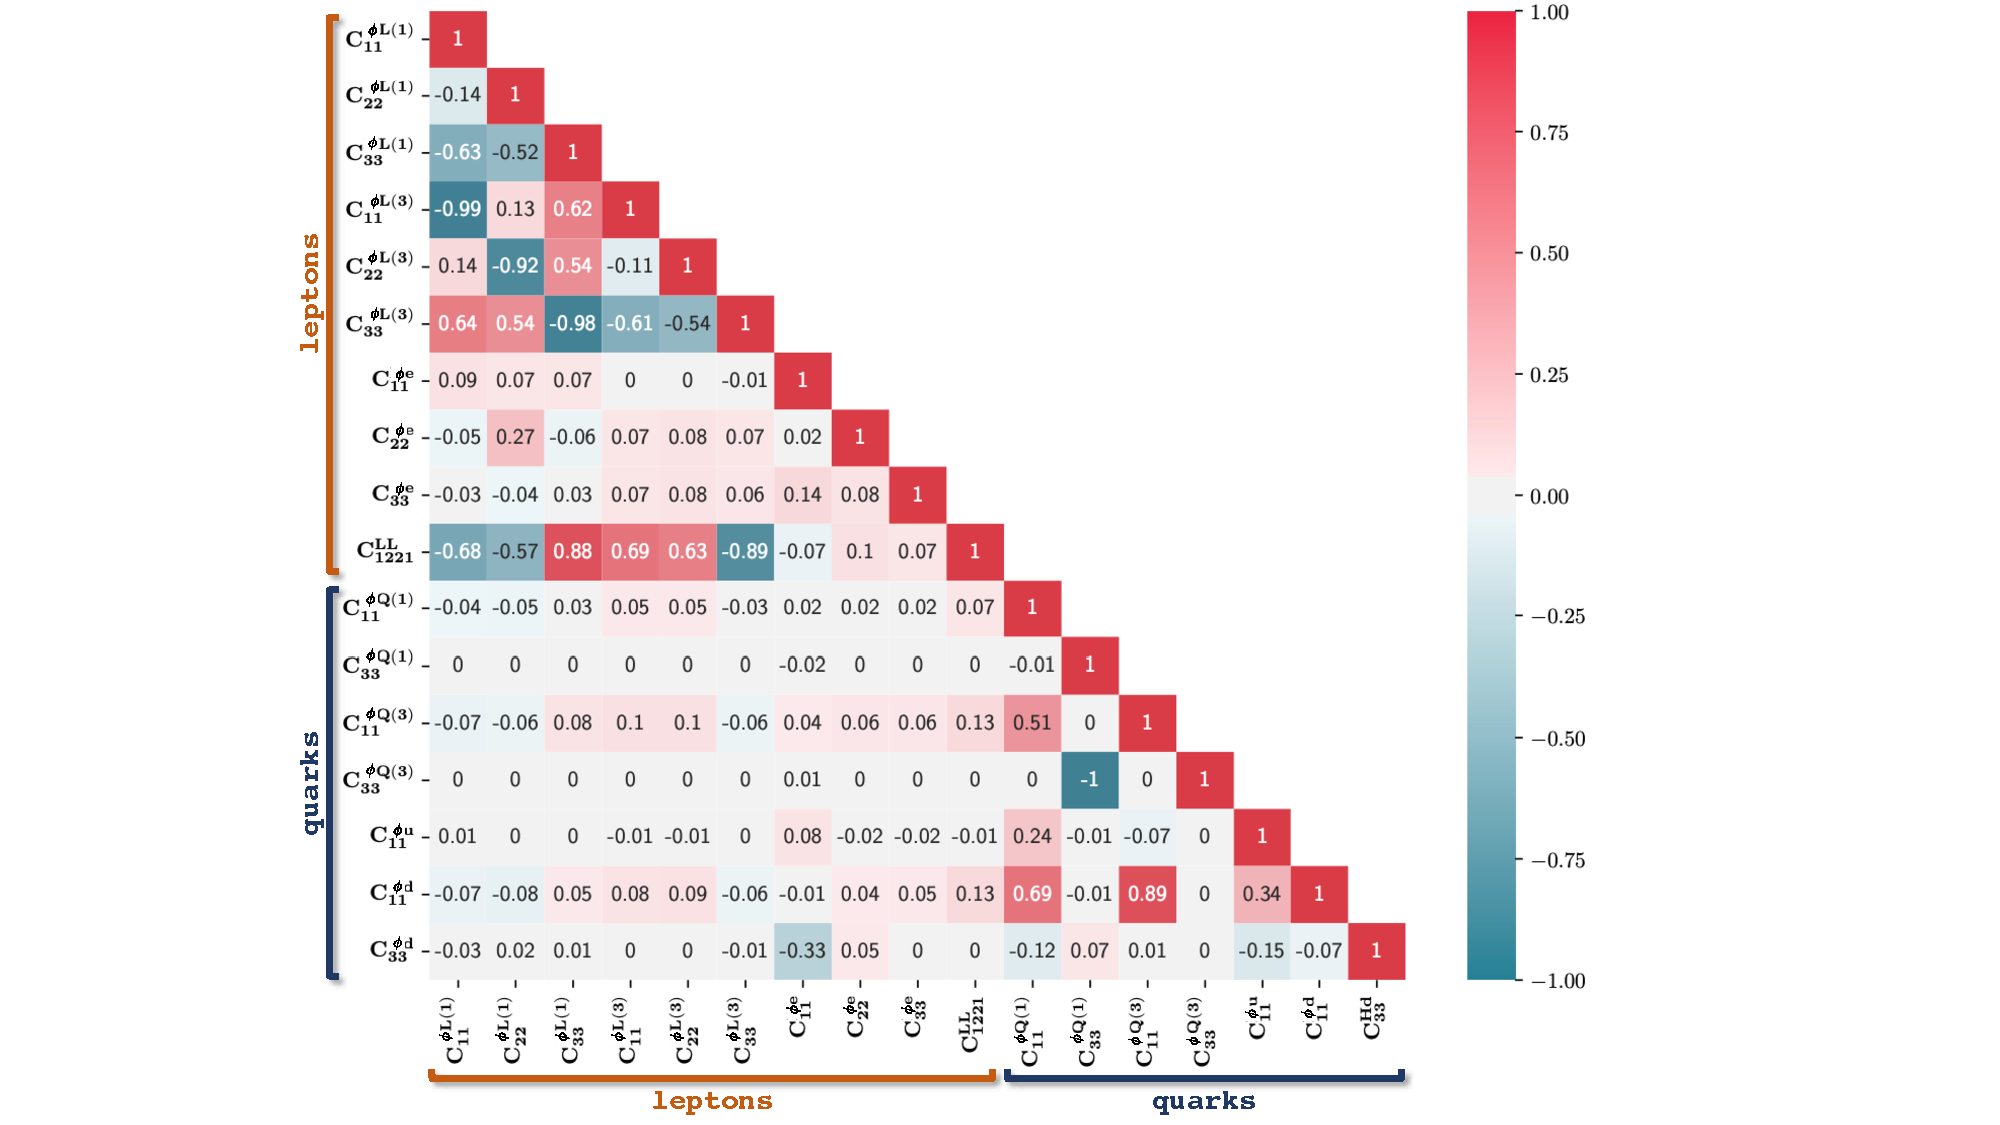
\includegraphics[width=\textwidth]{figures/heatmap_EW.pdf}
	\caption{\it The correlation matrix extracted from the SMEFT analysis of the set of independent operators in eqs.~\eqref{eq:SMEFT_op_HL}, \eqref{eq:SMEFT_op_HQ}, \eqref{eq:SMEFT_op_LLLL}, including only their effects at tree-level. The two distinct groups of correlated Wilson coefficients associated to leptonic and quark interactions are remarked as ``leptons'' and ``quarks'', respectively. Note that, compared to \autoref{fig:ew_corr}, in this tree-level analysis there is a significant decorrelation between the constraints on quarks and lepton operators.
	}
	\label{fig:ew_corr_tree}
\end{figure}

Here we revisit the constraints set by EWPO on the parameter space of the SMEFT. We make minimal flavour assumptions and include all quark and lepton operators described in the {\bf EW} fit presented in section~\ref{sec:strategy}. Measurements of EWPO have been extensively studied in the literature~\cite{Han:2004az,delAguila:2011zs,Ciuchini:2013pca,deBlas:2013gla,Falkowski:2014tna,Berthier:2015oma,Efrati:2015eaa,deBlas:2016nqo,deBlas:2017wmn,Ellis:2018gqa,Dawson:2019clf} within the SMEFT framework. The purpose here is to provide further details on the correlation between quark and lepton sectors constrained by EWPO, illustrating some of the effects when going beyond the tree-level analysis. 

The experimental inputs are the same considered for the {\bf EW} fit in section~\ref{sec:strategy}, and include, in particular, the full set measurements taken at LEP/SLD at the $Z$ pole, as well as the measurements of the $W$ boson obtained at LEP II, the Tevatron and the LHC (e.g. mass, width, branching ratios as well as the determination of $\left|V_{tb}\right|$ at the LHC~\footnote{The extraction of $\left|V_{tb}\right|$ could be, a priori, affected by other SMEFT effects entering in single-top production, e.g. 4-fermion operators. Such effects are neglected in our  analysis. The only effect of this input in the EW fits in this paper is to lift a flat direction that would otherwise appear between $C^{HQ^{(1)}}_{33}$ and $C^{HQ^{(3)}}_{33}$, had we excluded this measurement. Even with this input, these two coefficients are nearly $100\%$ correlated, as can be seen in \autoref{fig:ew_corr_tree}.}). For these fits we use the \HEPfit package~\cite{deBlas:2019okz} as for the rest of the work. 

\begin{figure}[t]
	\centering
	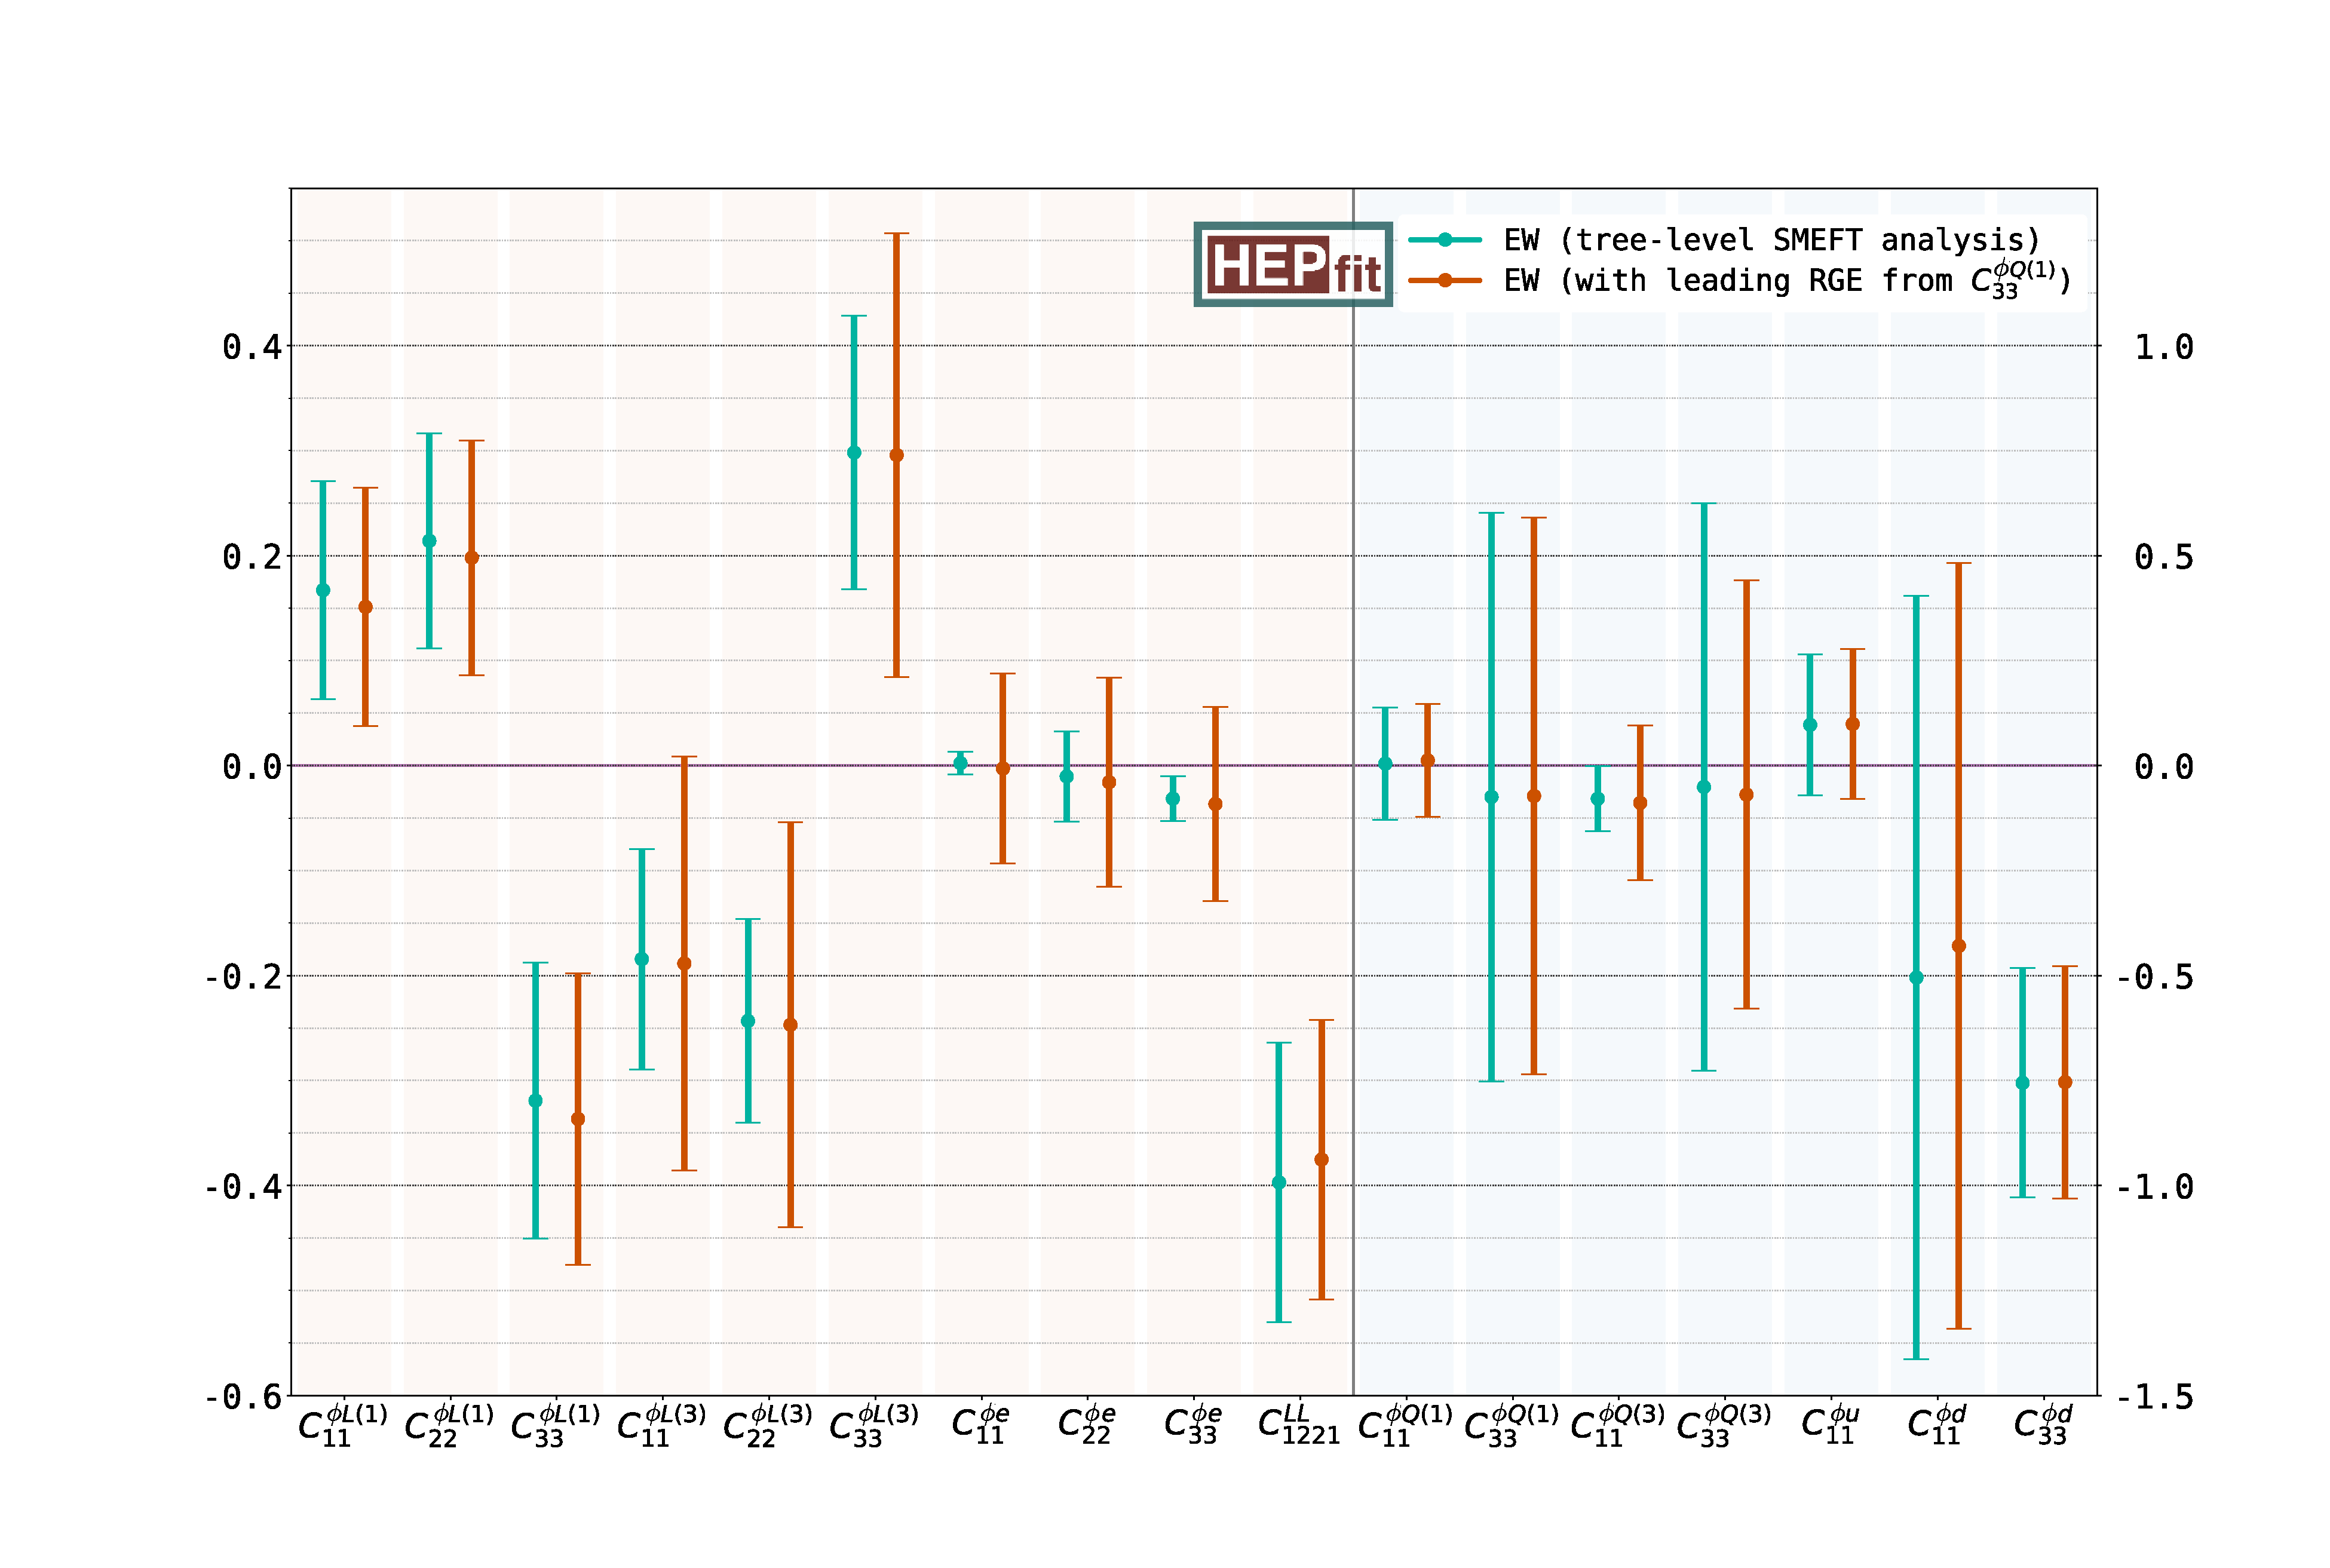
\includegraphics[width=\textwidth]{figures/errorbar_EW.pdf}
	\caption{\it Comparison of the mean and standard deviation of the marginalized posterior for the Wilson coefficients (in TeV$^{-2}$) of the operators included in the {\bf EW} fit under two different approximations: in green the results from a pure tree-level analysis; in orange we show the result including the dominant log-enhanced one-loop terms. See text for details. }
	\label{fig:ew_bounds}
\end{figure}

We first consider the case of the {\bf EW} fit at the tree level. In this case, the results of the fit reveal that while there is sizable correlation between the left-handed leptonic operators, as well as between the different quark operators, both sector are however decoupled to a good extent in the fit as can be seen from \autoref{fig:ew_corr_tree}.

For the main fits presented in section~\ref{sec:EFT_results}, however, we also consider the leading logarithmically enhanced contributions at one-loop level via RG running. For our purposes, and considering the size of the bounds on the different operators from the EW fit, the most important contribution comes from $C^{HQ^{(1)}}_{33}$. This induces an universal contribution that propagates into all EWPO. As a result of this, and similar to what was seen between the leptonic operators and the 4-fermion operators due to their interplay in eqs.~\eqref{eq:OLuedRGE}, a non-trivial pattern of correlations between the lepton and quark operator sectors in the {\bf EW} fit arises, as shown in \autoref{fig:ew_corr}. Similar to the change in the bounds on the leptonic operators in the {\bf EW+Flavour} fit once we included the RG effects of the four-fermion operators, the bounds on the leptonic operators also relax in the EW fit once we include the RG effects from $C^{HQ^{(1)}}_{33}$. This is shown in \autoref{fig:ew_bounds}. However, unlike in the {\bf EW+Flavour} fit, such effects do not induce a significant shift in the central values of the Wilson coefficients, which is simply due to the fact that the data selects $C^{HQ^{(1)}}_{33}$ to be centered around zero. 

As can be seen in \autoref{fig:ew_bounds}, the relaxation of the bounds can be in some cases rather dramatic, which brings about the question of what could be the impact of further effects not included in our analysis. We estimated that including the main RG effects for all the other operators in the EW fit amounts to changes of at most $\sim 25\%$. One should also note that finite terms involving the Wilson coefficients of the quark coupling may become relevant at this point. As can be deduced from the full NLO results presented in \cite{Dawson:2019clf}, these are not expected to significantly change the picture. In any case, the overall conclusions on this paper regarding the reconciliation between EW data and $B$ anomalies hold true.